\documentclass[]{article}
\renewcommand{\rmdefault}{ptm}
%\usepackage[hmargin=30mm]{geometry}
\usepackage{tabularx}
\usepackage{graphicx}
\usepackage{wrapfig}

\begin{document}

\begin{table}[here]
\centering
\begin{tabularx}{\textwidth}{| X | X | }
\hline
Topic of Survey								& 	Cloud Computing\\
\hline
Length of Survey							& 	15 pages\\
\hline
First team member's matriculation number	&	U096833E\\
\hline
First team member's name					&	LAURENCE PUTRA FRANSLAY\\
\hline
Sections done by first member				& 	1.1.x, 1.2.2\\
\hline
Second team member's matriculation number	&	\\
\hline
Second team member's name					&	\\
\hline
Sections done by second member				& 	\\
\hline

\hline
\end{tabularx}
\end{table}

\pagebreak

%9 pages
\section{Introduction to the various methods}
%fill in the method names as the subsection header
\subsection{MapReduce: Simplified Data Processing on Large Clusters}
\subsubsection{Introduction}
MapReduce, made popular by Google, is a programming model that is generally used to process and generate huge sets of data using distributed computing. It is based on 2 core functions of functional languages, \emph{map} and \emph{reduce}. Users of this model will first write a function that \emph{maps} a key-value pair to an intermediate key-value pair, and run this function on all the key-value pairs in the dataset. They will then write another function that aggregates all the values with the same key, and use it to \emph{reduce} the data to the output that is intended. \\

The code that runs the processing on large datasets using this programming model is generally \emph{embarrassingly parallel}\footnotemark\footnotetext{Embarassingly parallel programs are programs that have an almost perfect speed up because each component can be done individually.}, and hence, this programming model is often utilised to process large data sets on multiple computers and sometimes even multiple datacenters. \\

\subsubsection{How it works}
MapReduce is generally available as a library, where the users supply the \emph{map} and \emph{reduce} functions, as well as the input data. The \emph{map} function, which is written by the user, takes in a set of key-value pair, processes it, and returns a set of intermediate key-value pairs. After the final set of intermediate key-value pair has been generated, the intermediate data set is then passed to the \emph{reduce} function. The \emph{reduce} function will then process all the values with the same key, generating a final result for that key that takes into account all the values that key has.\\

The \emph{map} and \emph{reduce} functions are generally put into a larger MapReduce system that handles more of the backend processing, including allocating the tasks to the machine, and aggregating all the results to return after \emph{reduce} has completed the post processing.\\


\subsubsection{Implementation}
There are various ways to implement MapReduce, and it generally depends on the hardware available, and the following describes the implementation that is done at Google. However, in general, MapReduce is run on distributed systems, and generally on warehouse scale machines.\\

The data is first split into chunks of 16MB to 64MB, dependent on user input, due to the fact that the filesystem is stored in 64MB chunks, and the program is started up multiple times on the cluster that is assigned for that task. Of all the copies of the program that is started up, one of it would be assigned the master role, and has the job of assigning idle workers to a task. When an idle worker is assigned a \emph{map} task, it will then process the corresponding chunk of data, and pass each key-value pair to the \emph{map} function. The intermediate key-value pairs produced by the \emph{map} function is then temporarily stored in memory. The intermediate key-value pairs stored in memory are then regularly pushed onto local storage, and their stored locations are then passed to the master program to keep track of. The master program will then assign \emph{reduce} tasks to the worker programs, who will sort the intermediate data based on their key's before performing the actual processing. If the amount of data is too large, it will sometimes be done externally by another program. After this processing is completed, the reduce function will process the sorted intermediate data, and return the output and write it to a global storage. Once all the map tasks and reduce tasks are finally completed, the master program will wake up the user program and continue processing in the user program. The result of the MapReduce call will be be available in the \emph{n} output files generated by the \emph{n} reduce tasks, and would generally be fed as input to another MapReduce function call.\\

As the master program is central to a MapReduce operation succeeding, it will have to store the state of each \emph{map} and \emph{reduce} task, as well as the machine the task is running on. The master program also has to store the location and size of the results of each map task that is written to local storage so that the \emph{reduce} tasks are able to find the intermediate data set. \emph{Reduce} tasks that are already running are also given updates when there are any. \\

\subsubsection{Fault tolerance}
The MapReduce library is intended to process a massive amount of data using massive computational resources. Hence, there is a requirement to make this system able to recover from faults too. However, it is worth noting in this case that Google is actually using a custom filesystem, that has the ability to recover from hardware failure due to it's usage of redundancy.\\

First, the master program will have to ensure that  the worker programs are working. If any of the worker programs fail, the master program will have to assign another worker program to handle the task that has failed, regardless of whether it is the \emph{map} or \emph{reduce} functions. The master does this by pinging the worker programs at regular intervals. If the worker program does not respond, the master program then takes it that the worker program has failed, and then marks all \emph{map} tasks that have been processed or being processed by that worker program as unprocessed, and will then assign other worker programs to handle those tasks. This is as the processed data is stored on local storage, and not in global storage, the rest of the system will not be able to access the data in the failed machine. The workers handling the reduce tasks will also be informed of the reexecution of the \emph{map} task, so that the tasks that have yet to get the data from the now failed system can get it from the new system in charge of that \emph{map} task. However, \emph{reduce} tasks do not need to be redone on failure as the results from the \emph{reduce} tasks are store in global storage.\\

In the event of the failure of the master program, things are done differently. Google will abort the computation when the master program has failed, and letting the clients do the checks and deciding if they should retry, simply because this happens very rarely (only 1 program out of the possible thousands is the master). However, if someone wants to make it failsafe, one can simply make the master commit the state to the global storage (which is redundant and failsafe), and then spin up another master program when it goes down and start again from the state stored in the global storage.\\

One unique and defining attribute of the MapReduce library is that if the \emph{map} and \emph{reduce} functions are deterministic based on the input values, the program will generate the exact same result that is generated by a sequential execution of the entire program. In order to achieve this, every \emph{map} and \emph{reduce} tasks have atomic commits. Each \emph{map} task takes in 1 file, and produces \emph{n} files, where \emph{n} is the number of \emph{reduce} tasks. When the \emph{map} task finishes, it will send a message to the master program, together with the locations of the \emph{n} output files. The master program will then check if this current \emph{map} task has been completed before. If not, it will then store the locations of the \emph{n} files in it's state. The \emph{reduce} program, on the other hand, is slightly different. It will rename it's temporary output file to the final output file atomically, and uses the file system to guarantee that the state in the filesystem only contains the data produced by a single \emph{reduce} task. As a result of these properties, the program is fairly fault tolerant.\\

\subsubsection{Reducing I/O}
In order to reduce network bandwidth, which is generally a scarce resource in most datacenters, the MapReduce master program will assign \emph{map} tasks onto input values that it is in close proximity to, preferably the same machine. This would ensure minimal amounts of network I/O. \\ 

\subsubsection{How tasks are divided}
Assume we that the input data is spilt into $X$ parts, and there are $Y$ reduce tasks. Under most circumstances, the following equation should hold: $X + Y > no. of machines$, and even far exceed the number of machines. This is as allowing each machine to perform multiple tasks would firstly improve load balancing, as machines performing longer tasks can then be assigned less tasks, and secondly, allow for faster recovery from failure as the many tasks done by that machine can now be split between the many machines.\\

However, while theoretically, the more tasks we have the better, we have to keep in mind that the scheduling and load balancing is handled by the master program. If we have too many tasks, the complexity of scheduling of the tasks increases with each new task added. \\

In addition to that, as each \emph{reduce} task ends up generating it's own output file, and the user will have to read each output file, either programmatically or manually, $Y$ is often not very large, generally taking a small integer multiplied by the total number of machines. However, in the case of $X$, generally the tasks are spilt such that each task will take in a fixed amount of data that is optimal for reducing I/O.\\

\subsubsection{Reducing Outliers}
In addition to most of the methods listed above, there are times when certain tasks take way longer than expected to run, and lengthens the total running time for the MapReduce operation. This could be due to hardware failure, or some other non-MapReduce programs running some computationally-intensive task on that machine, or some other problem. \\

A general method used by MapReduce to counter this kind of issues is to run redundant tasks when a large number of it's worker machines are idle and not processing anything related to the MapReduce operation. When the MapReduce operation is almost completed and there are a few straggler tasks that are running, the master program will allocate identical tasks to a other machines as well, and the task is considered completed when any one of the machines has completed the task. \\

\subsubsection{Addons to the MapReduce library}
There has been some additions made to the MapReduce library on top of the basics as detailed above.\\

Firstly, the users of the library can not only define the number of \emph{map} and \emph{reduce} tasks, but also the way the output data is partitioned. This is especially useful in cases where the hierarchical string, and only a certain part of the string should be taken as the identifier when partitioning.\\

Another addon which may come in useful to most users is that the partition files are sorted in ascending order. This would allow future users of the file to easily look for the data they require within the file. \\

A useful addon to reduce network I/O would be the combiner. In essence the combiner just runs the \emph{reduce} function right after \emph{map}, and write it to the intermediate output file. For example, in a program that counts the total number of words there are might have plenty of duplicate words due to the map function. What the combiner  would do is to merge this data together first so that instead of sending thousands of records over, it can be sent as a few records.\\

\subsection{Additional enhancement to MapReduce}
%each of these sections should take around 1.5 to 2 pages.
\subsubsection{Camdoop}
%Preprocessing instead of post processing





\subsubsection{Mantri}
% Load balancing tasks and reduce the effects caused by outliers
Mantri is a method that use used to reduce the impact that outliers have on the entire MapReduce operation. As detailed earlier, MapReduce internally handles outliers by assigning an identical task to another worker machine, in the hopes that it can complete the task earlier. These outliers may happen due to many reasons, including but not limited to heavy workload for that machine, or large quantities of hard disk I/O during that period of time. \\

Mantri works on reducing the amount of impact outliers have on the system by identifying the main causes for such outliers, which is mainly high hard disk I/O, congested network pipes, as well as a skewed assignment of task as a result of the data partitioning which is often done over a set of data that is not exactly random. Mantri has been tested on all of Bing's production cluster and has shown to have large performance benefits, speeding up more than half the jobs by 50\%. \\

Mantri basically identifies certain checkpoints that the tasks are not able to perform at the expect rate, and solves these issues by trying to solve the underlying issue causing the slowdown in performance. The figure below shows the actions taken by Mantri for each type of problem. \\
\begin{figure}[here]
	\begin{center}
		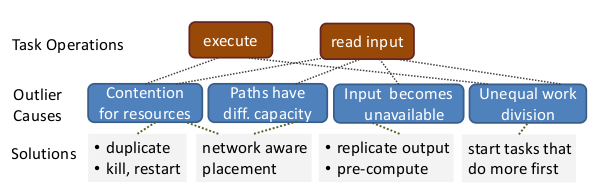
\includegraphics[width=0.9\textwidth]{mantri11.png}
		\caption{Actions taken by Mantri}
	\end{center}
\end{figure}

The first targeted solution for Mantri is restarting the task. There are 2 forms of restart that Mantri uses. The first form is to kill the existing running task and to restart it somewhere else. The other form is to duplicate the existing task and run it elsewhere. The restart solution kicks in only when there is a high chance that the time taken for the new task to complete is smaller than the time remaining for the current task to complete. However, restarting a task would require computational resources, this is only done when there are idle worker machines. When more spare jobs are available, Mantri will then schedule duplicates a little more aggressively.\\

The second targeted solution is to place tasks in such a way that it is aware of the network environment around it. As shown in section $1.1.3$, \emph{reduce} tasks will first have to read the intermediate files generated by the various \emph{map} tasks. If a server rack has too many \emph{reduce} tasks, it's incoming network would very likely be congested, and this would have a detrimental effect on all the \emph{reduce} tasks running on the rack. Using Mantri, the programs that manage the tasks will locate the task on the worker machines based while trying to reduce the load on the network, and try to prevent the various tasks from mutually interfering. It has an algorithm that figures out which is the optimal location to place all the tasks based on network bandwidth, in such a way such that the maximum data transfer time is minimized.\\

The third targeted solution is to avoid recomputations. As mentioned in the earlier section on MapReduce, the MapReduce library will store the output of \emph{map} tasks on local storage, and hence when the machine fails, the output is gone, and recomputation would need to be redone. In this case, Mantri will replicated the output data in tasks whose recomputation costs are higher than the replication costs. The recomputation costs is calculated by taking the product of the probability that the machine will fail with the estimated time for the task to be recomputed. The estimated time to recompute is calculated taking into account that the input is lost as well. For example, in a \emph{reduce} task, which takes in a large number of input, the estimated time to recomputate would be higher as recomputing the intermediate data to feed to the \emph{reduce} task as input data will stall the operation as a whole. In essence, the output is replicated when $1)$ the cummulative costs of not replicated consecutive task increases, or $2)$ when the machines used are really unstable, or $3)$ when the output is really small such that the cost of replication is neglible. However, it is worht noting that Mantri will enforce a limit on the amount of data to be replicated to up to 10\%. Each job will have a token proportional to the data processed, and if the cost benefit check is satisfactory for replication, the replication is done only when there are sufficient tokens available, and the tokens are deducted on replication of data.\\

In addition, the task ordering by Mantri will take into account the size of each task. It will schedule the longer tasks first, and run the smaller tasks last, so that it is at most 33\% slower than the optimal schedule, which is NP-hard to compute.\\

The tasks will also estimate the time remaining via the following equation. 

$time_{remaining} = time_{elapsed} * \frac{data}{data_{read}} + time_{wrapup}$

Mantri uses a moving average, and in order to handle lost reports, if a task has not reported for some time, $time_{remaining}$ is automatically increased, with the assumption that no progress has been made.

\subsubsection{Nectar}

\subsubsection{Optimising data shuffling in Data Parallel Computation}

%3 pages
\section{Advantages and Disadvantages of each method}
%fill in the method names as the subsection header
\subsection{}

\subsection{}

\subsection{}

\subsection{}

\subsection{}

%1 page
\section{Creating a more robust combination}

%1 page
\section{State of Research}

\end{document}